%%%%%%%%%%%%%%%%%%%%%%%%%%%%%%%%%%%%%%%%%
% Beamer Presentation
% LaTeX Template
% Version 1.0 (10/11/12)
%
% This template has been downloaded from:
% http://www.LaTeXTemplates.com
%
% License:
% CC BY-NC-SA 3.0 (http://creativecommons.org/licenses/by-nc-sa/3.0/)
%
%%%%%%%%%%%%%%%%%%%%%%%%%%%%%%%%%%%%%%%%%

%----------------------------------------------------------------------------------------
%	PACKAGES AND THEMES
%----------------------------------------------------------------------------------------

\documentclass{beamer}

\mode<presentation> {

% The Beamer class comes with a number of default slide themes
% which change the colors and layouts of slides. Below this is a list
% of all the themes, uncomment each in turn to see what they look like.

%\usetheme{default}
%\usetheme{AnnArbor}
%\usetheme{Antibes}
%\usetheme{Bergen}
%\usetheme{Berkeley}
%\usetheme{Berlin}
%\usetheme{Boadilla}
%\usetheme{CambridgeUS}
%\usetheme{Copenhagen}
%\usetheme{Darmstadt}
%\usetheme{Dresden}
%\usetheme{Frankfurt}
%\usetheme{Goettingen}
%\usetheme{Hannover}
%\usetheme{Ilmenau}
%\usetheme{JuanLesPins}
%\usetheme{Luebeck}
\usetheme{Madrid}
%\usetheme{Malmoe}
%\usetheme{Marburg}
%\usetheme{Montpellier}
%\usetheme{PaloAlto}
%\usetheme{Pittsburgh}
%\usetheme{Rochester}
%\usetheme{Singapore}
%\usetheme{Szeged}
%\usetheme{Warsaw}

\usepackage{lipsum}
\usepackage{hyperref}
\hypersetup{
    colorlinks=true,
    linkcolor=white,
    filecolor=blue,      
    urlcolor=blue,
}
% As well as themes, the Beamer class has a number of color themes
% for any slide theme. Uncomment each of these in turn to see how it
% changes the colors of your current slide theme.

%\usecolortheme{albatross}
%\usecolortheme{beaver}
%\usecolortheme{beetle}
%\usecolortheme{crane}
%\usecolortheme{dolphin}
%\usecolortheme{dove}
%\usecolortheme{fly}
%\usecolortheme{lily}
%\usecolortheme{orchid}
%\usecolortheme{rose}
%\usecolortheme{seagull}
%\usecolortheme{seahorse}
%\usecolortheme{whale}
%\usecolortheme{wolverine}

%\setbeamertemplate{footline} % To remove the footer line in all slides uncomment this line
%\setbeamertemplate{footline}[page number] % To replace the footer line in all slides with a simple slide count uncomment this line

%\setbeamertemplate{navigation symbols}{} % To remove the navigation symbols from the bottom of all slides uncomment this line
}

\usepackage{graphicx} % Allows including images
\usepackage{booktabs} % Allows the use of \toprule, \midrule and \bottomrule in tables

%----------------------------------------------------------------------------------------
%	TITLE PAGE
%----------------------------------------------------------------------------------------

\title[daycare solution]{Mobilní aplikace pro pracovníky pečovatelské služby} % The short title appears at the bottom of every slide, the full title is only on the title page

\author{Petr Janiš} % Your name
\institute[UPOL] % Your institution as it will appear on the bottom of every slide, may be shorthand to save space
{
Univerzita Palackého v Olomouci
\\ % Your institution for the title page
\medskip
}
\date{18.6.2020} % Date, can be changed to a custom date

\begin{document}

\begin{frame}
\titlepage % Print the title page as the first slide
\end{frame}

\begin{frame}
\frametitle{Motivace pro tvorbu aplikace}
\begin{itemize}
\item {\large Sociální služby v ČR vs zahraničí}\\[3mm]
\item {\large Požadavky státních organů}\\[3mm]
\item {\large Usnadnění pracé zaměstnancům}\\[3mm]
\item {\large Celý proces SW vývoje}
\end{itemize}
\end{frame}


\begin{frame}
\frametitle{Použité technologie}
\begin{itemize}
\item {\large .NET Core}\\[3mm]
\item {\large Angular}\\[3mm]
\item {\large Docker}\\[3mm]
\item {\large Azure $\Rightarrow$ Hosting, CI}
\end{itemize}
\end{frame}


\begin{frame}
\frametitle{Návrh systému}
\vspace{7mm}
\begin{figure}[center]
  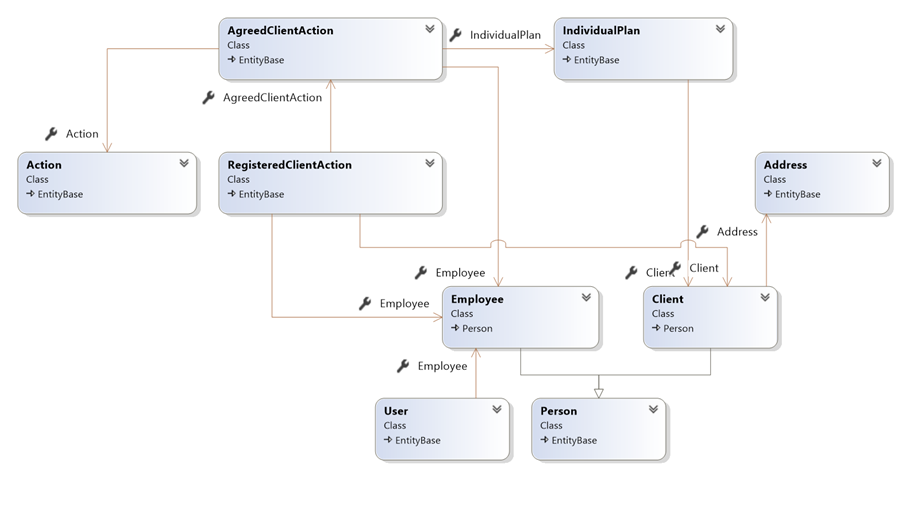
\includegraphics[width=12cm]{obr2.png}
  \label{fig:Github}
\end{figure}
\end{frame}

\begin{frame}
\frametitle{Plány do budoucna}
\begin{itemize}
\item {\large Rozšířit možnosti autentizace (Biometrika, Refresh)}\\[3mm]
\item {\large  gRPC (chat, poloha zařízení)}\\[3mm]
\item {\large Push notifikace}\\[3mm]
\item {\large PWA}\\[3mm]
\item {\large UI- aplikace pro mobilní pečovatele}
\end{itemize}
\end{frame}


\begin{frame}
\frametitle{Demo}
\begin{itemize}
\item {\large \href{https://daycaress-api-test.azurewebsites.net/index.html}{https://daycaress-api-test.azurewebsites.net/index.html}
}\\[3mm]

\item {\large \href{https://dayss-clients.azurewebsites.net/\#/login}{https://dayss-clients.azurewebsites.net/\#/login}
}\\[3mm]

\item {\large \href{http://dayss-clients.azurewebsites.net/manager_app/\#/manager_app/login}{http://dayss-clients.azurewebsites.net/manager\_app/\#/manager\_app/login}
}\\[3mm]
\end{itemize}
\end{frame}

\begin{frame}
\frametitle{Posudek vedoucího (1/2)}
\begin{itemize}
\item Mobilní aplikaci jsem testoval na platformně Android – aplikace je funkční, avšak trpí
menšími "nenativními neduhy", které však nezkušený uživatel nejspíš nepostřehne (do
textového pole pro komentář akce u klienta lze hůře psát text, uložení akce při běžících
stopkách ukáže NaN, selhání navigace pomocí aplikace Mapy.cz by mohlo být oznámeno,
piny na mapě s fotkami studentů si při zoomování neudržují přesnou polohu a mírně se
posunují).

\item větší přehlednost na větších obrazovkách. V odevzdané uveřejněné verzi se mi nenačetla
mapa.
\end{itemize}
\end{frame}
\begin{frame}
\frametitle{Posudek vedoucího (2/2)}
\begin{itemize}
\item Při listování kalendářem načtení nového měsíce trvá déle a uživatel o načítání není
nijak vizuálně informován, tedy může nabýt dojmu, že se aplikace zasekla.
\item Designově není aplikace příliš přívětivá – je vidět, že jsou použity barvy výchozí
šablony. Dle mého názory by aplikace měla být formálnější.
\item Při přesouvání akcí v individuálním plánu klienta není dodrženo místo, kam byla
akce přesunuta. Vždy uskočí o dvě hodiny.
\end{itemize}
\end{frame}

\begin{frame}
\frametitle{Posudek oponenta (1/2)}
\begin{itemize}
\item Autor v práci píše: "Je tedy potřeba nejdříve spustit stránku s API v prohlížeči a počkat
na načtení." Připadá mi poněkud náročné pro uživatele, aby po instalaci mobilní
aplikace musel ještě ručně spouštět stránku s API. Nešlo by to udělat tak, aby aplikace
fungovala hned po instalaci?

\item Při každém spuštění potřebuje aplikace stahovat data ze serveru. Toto trvá poměrně
dlouho i při připojení pomocí WiFi. Vzhledem k tomu, že aplikace je určena
především k práci v terénu, je toto dost nepraktické. Nešlo by mít data uložena přímo
v aplikaci a minimalizovat přenos data se serverem, případně tento přenos odložit až
na dobu, kdy bude k dispozici připojení k Internetu?

\item  Užitečnou funkcí je sledování trvání jednotlivých akcí. Toto je ale trochu utopeno
přímo v popisu akce. Nešlo by upozornění na běžící sledování trvání akce umístit
někam viditelněji?
\end{itemize}
\end{frame}

\begin{frame}
\frametitle{Posudek oponenta (2/2)}
Pro manažery slouží webová aplikace, která umožňuje vytvářet klientům účty a individuální
plány. Aplikace vypadá pěkně a její ovládání je intuitivní. Při jejím používání jsem však
narazil na množství problémů:
\\[4mm]
\begin{itemize}
\item Když jsem klientovi vytvořil individuální plán a nastavil jednotlivé akce, toto se vůbec
nezobrazilo v rozpisu akcí a ani se to nepromítlo v mobilní aplikaci zaměstnance.
\item Vytváření akce funguje velmi divně. Pokud akci přetáhnu do plánu např. na 5:00, po
uložení se naplánuje od 7:00. Na ruční úpravu času aplikace vůbec nereaguje.
Obdobně špatně funguje přetažení akce v plánu.
\item Připadá mi poněkud nepraktické mít možnost vytvořit jen pravidelný rozpis akcí na
kalendářní týden. Při péči o klienty se nikdy nevyskytne jednorázová akce? 
\end{itemize}
\end{frame}

%----------------------------------------------------------------------------------------

\end{document} 